\documentclass[../../main]{subfiles}

\begin{document}
\chapter{数ベクトル空間}
\label{chapter:numerical_vector_space}

\begin{lead}
  \cref{chapter:numerical_vector_space}では,数ベクトル空間における直交性と最良近似の関係を説明する.
\end{lead}

\section{イントロダクション}
\label{section:numerical_vector_space_introduction}

\cref{chapter:numerical_vector_space}では,数ベクトル空間\(\numset{K}^n\)(\(\numset{K}=\numset{R},\numset{C}\))に関する理論を扱う.
信号解析において,この理論は
\begin{enumerate}
  \item 離散時間信号の時系列分析
  \item 観測値をモデルに対応づける回帰・判別分析
\end{enumerate}
という,2つの方向に応用される.

音声信号処理は前者の主要な例である.音声信号を計算機で処理するには,時々刻々と値が変わる信号を有限長のデータで表現しなければならない.
たとえば,CDでは音声信号の瞬時値を1秒あたり44100個記録している.すなわち,時刻\(t\)秒における瞬時値を\(x(t)\),収録時間を\(T\)秒とおくと,CDには数列\(\seq{x(n/44100)}_{n=0}^{44100T}\)が記録されている.
そこで,収録されたデータを\(\numset{R}^{44100T+1}\)の元とみなせば,\(\numset{R}^n\)に関する理論に基づいて音声を解析できる.

後者の主要な例は最小2乗法である.実験で得られた標本を理論と見比べるとき,理論から得られる式へのあてはめ(回帰)がしばしば試される.
あてはまりのよさを示す指標はいろいろあるが,最もポピュラーなのは2乗誤差を指標にする最小2乗法である.本書ではこの最小2乗法を,内積と関連づけ幾何的に説明する.

\section{直交射影}

本節では,あるベクトルを他のベクトルの線型結合で近似する手法を説明する.
特に断りのない限り,\cref{chapter:numerical_vector_space}において\(\numset{K}\)は\(\numset{R}\)か\(\numset{C}\)を意味し,
\(\innerp{\holder}{\holder}\)は\(\numset{K}^n\)の標準内積を意味する.また
\[
  \vnorm{\vect{x}} = \sqrt{\innerp{\vect{x}}{\vect{x}}}
  = \sqrt{\abs{x_1}^2+\dots+\abs{x_n}^2}
  \quad(\vect{x}=\trps{\matrice{x_1 & \cdots & x_n}}\in\numset{K}^n)
\]
とする\indexsymbol{\(\vnorm{\holder}\)}.

\subsection{直交射影}

\begin{wrapfigure}[8]{o}{0pt}
  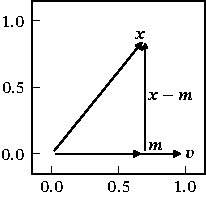
\includegraphics{figures/proj2d.pdf}
\end{wrapfigure}

\(\numset{K}^n\)のベクトル\(\vect{x}\),部分空間\(V\)が与えられたとき,\(V\)の元で\(\vect{x}\)に最も近いベクトル,すなわち,距離\(\vnorm{\vect{x}-\vect{m}}\)を最小にする\(\vect{m}\in V\)について考えよう.

\(\numset{K}^n\)が平面\(\numset{R}^2\)で,\(V\)があるベクトル\(\vect{v}\neq\zvec\)により生成される直線\(\spannedby\Set{\vect{v}}\)の場合,\(\vect{m}\)は図の位置にある.
図を見ると,\(\vect{x}-\vect{m}\)は\(\vect{v}\)と直交しているのが分かる.

一般の部分空間\(V\subset\numset{K}^n\)においても,直交性と最良近似には密接な関係がある.その証明へと入る前に,便利な記法を2つ定義しておく.

\begin{definition}{argmin,argmax}{argmin_argmax}\index{argmin@\(\argmin f(x)\)}\index{argmax@\(\argmax f(x)\)}
  実数値関数\(f\)は集合\(S\)を定義域に含むとする.\(S\)の部分集合\(\argmin_{x\in S}f(x)\),\(\argmax_{x\in S}f(x)\)を以下の通り定義する.
  \begin{gather*}
    \argmin_{x\in S}f(x) = \Set{x\in S\given\text{任意の\(y\in S\)に対して\(f(y)\geq f(x)\)}}, \\
    \argmax_{x\in S}f(x) = \Set{x\in S\given\text{任意の\(y\in S\)に対して\(f(y)\leq f(x)\)}}
  \end{gather*}
\end{definition}

\cref{definition:argmin_argmax}からただちに,次のことが分かる.

\begin{proposition}{}{}
  \(S\)の元\(a\)に関する以下の条件は同値であり,同様のことが\(\argmax\)についても成り立つ.
  \begin{enumerate}
    \item \(a\in\argmin_{x\in S}f(x)\)である.
    \item \(f(a)\)は集合\(\ran{f}{S}=\Set{f(x)\given x\in S}\)の最小元である.
  \end{enumerate}
\end{proposition}

\begin{wrapfigure}[8]{o}{0pt}
  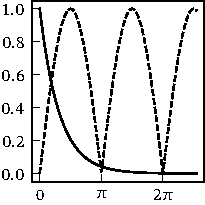
\includegraphics{figures/argmin.pdf}
\end{wrapfigure}

図は\(\napr^{-x}\)と\(\abs{\sin x}\)のグラフである.\(\napr^{-x}\to 0\)(\(x\to\infty\))であるが,\(\napr^{-x}=0\)となる実数\(x\)は存在しない.そのため
\begin{gather*}
  \argmin_{x\in\coival{0}{\infty}}\napr^{-x} = \emptyset\quad\text{(空集合)}, \\
  \argmin_{x\in\coival{0}{\infty}}\abs{\sin x} = \Set{0,\krez,2\krez,\dotsc}
\end{gather*}
である.このように,\(\argmin_{x\in S}f(x)\)は空になることも,無限集合になることもある.

\(\numset{K}=\numset{R}\)の場合も同様に証明できるので,\cref{proposition:finite_projection}まで証明では\(\numset{K}=\numset{C}\)を仮定する.また,部分空間が\(\Set{\zvec}\)でないことも仮定する.

\begin{lemma}{}{binomial_square}
  各\(\vect{x},\vect{y}\in\numset{K}^n\)に対して\(\vnorm{\vect{x}+\vect{y}}^2=\vnorm{\vect{x}}^2+2\rpart\innerp{\vect{x}}{\vect{y}}+\vnorm{\vect{y}}^2\)が成立する.
\end{lemma}

\begin{proof}
  \(\vnorm{\vect{x}+\vect{y}}^2=\innerp{\vect{x}+\vect{y}}{\vect{x}+\vect{y}}\)の右辺を展開すれば示せる.
\end{proof}

\begin{proposition}{}{finite_convex_projection}
  \(\vect{x}\in\numset{K}^n\)かつ,\(V\)は\(\numset{K}^n\)の部分空間とする.
  このとき,\(\argmin_{\vect{y}\in V}\vnorm{\vect{x}-\vect{y}}\)はただ1つの元からなる集合である.
\end{proposition}

\begin{proof}
  本証明に限り,\(\sum_{k=1}^m\)(\(m=\dim V\))を\(\sum\)と略記する.\(\basis{B}=\Set{\vect{e}_1,\dots,\vect{e}_m}\)を\(V\)の正規直交基底とする.
  このとき\(V=\Set{\sum z_k\vect{e}_k\given z_1,\dots,z_m\in\numset{C}}\)なので,\(\epsilon(z_1,\dots,z_m)=\vnorm{\vect{x}-\sum z_k\vect{e}_k}\)とおくと
  \[
    \argmin_{\vect{y}\in V}\vnorm{\vect{x}-\vect{y}} = \Set*{\sum z_k\vect{e}_k\given\trps{\matrice{z_1 & \cdots & z_m}}\in\argmin_{\vect{z}\in\numset{C}^m}\epsilon(\vect{z})}
  \]
  である.

  \(\argmin_{\vect{z}\in\numset{C}^m}\epsilon(\vect{z})\)を求める.\(\innerp{\vect{e}_i}{\vect{e}_j}=\kdelta{i}{j}\)だから
  \[
    \vnorm*{\sum_{i=1}^mz_i\vect{e}_i}^2 = \innerp*{\sum_{i=1}^mz_i\vect{e}_i}{\sum_{j=1}^mz_j\vect{e}_j}
    = \sum_{i=1}^mz_i\sum_{j=1}^m\conj{z}_j\innerp{\vect{e}_i}{\vect{e}_j}
    = \sum_{i=1}^mz_i\conj{z}_i
    = \sum_{i=1}^m\abs{z_i}^2
  \]
  である.したがって,\cref{lemma:binomial_square}より
  \begin{align*}
    \epsilon(\vect{z})^2 &= \vnorm*{\vect{x}-\sum z_k\vect{e}_k}^2 = \vnorm{\vect{x}}^2-2\rpart\innerp*{\vect{x}}{\sum z_k\vect{e}_k}+\vnorm*{\sum z_k\vect{e}_k}^2 \\
    &= \vnorm{\vect{x}}^2-2\sum\rpart[\conj{z}_k\innerp{\vect{x}}{\vect{e}_k}]+\sum\abs{z_k}^2
  \end{align*}
  である.よって,\(\epsilon(\vect{z})^2\)は\(s_k=\rpart z_k\)と\(t_k=\ipart z_k\)の式で
  \begin{align*}
    \epsilon(\vect{z})^2 &= \vnorm{\vect{x}}^2+\sum(-2\rpart[(s_k-\iuni t_k)\innerp{\vect{x}}{\vect{e}_k}]+s_k^2+t_k^2) \\
    &= \vnorm{\vect{x}}^2+\sum(-2(s_k\rpart\innerp{\vect{x}}{\vect{e}_k}+t_k\ipart\innerp{\vect{x}}{\vect{e}_k})+s_k^2+t_k^2) \\
    &= \vnorm{\vect{x}}^2+\sum((s_k-\rpart\innerp{\vect{x}}{\vect{e}_k})^2+(t_k-\ipart\innerp{\vect{x}}{\vect{e}_k})^2-\abs{\innerp{\vect{x}}{\vect{e}_k}}^2)
  \end{align*}
  と書けるので,次式が成立する.
  \begin{equation}
    \label{equation:pre_bessels_inequality}
    \epsilon(\vect{z})^2 = \vnorm{\vect{x}}^2+\sum_{k=1}^m\abs{z_k-\innerp{\vect{x}}{\vect{e}_k}}^2-\sum_{k=1}^m\abs{\innerp{\vect{x}}{\vect{e}_k}}^2
  \end{equation}

  \cref{equation:pre_bessels_inequality}より\(\argmin_{\vect{z}\in\numset{C}^m}\epsilon(\vect{z})=\Set{\trps{\rowvect{\innerp{\vect{x}}{\vect{e}_1} & \cdots & \innerp{\vect{x}}{\vect{e}_m}}}}\)であるから,
  \(\argmin_{\vect{y}\in V}\vnorm{\vect{x}-\vect{y}}=\Set{\sum\innerp{\vect{x}}{\vect{e}_k}\vect{e}_k}\)である.
\end{proof}

なお,\cref{proposition:finite_convex_projection}は部分空間よりも少し広い対象(閉凸集合)へと一般化できるのだが,そのことは\cref{xr-chapter:hilbert_space}であらためて扱う.

\begin{proposition}{}{weak_finite_projection}
  \(\vect{x}\in\numset{K}^n\)かつ,\(V\)は\(\numset{K}^n\)の部分空間とする.
  \(V\)のある元\(\vect{m}\)が任意の\(\vect{v}\in V\)に対し\(\innerp{\vect{x}-\vect{m}}{\vect{v}}=0\)を満たすとき,
  \(\vect{m}\in\argmin_{\vect{y}\in V}\vnorm{\vect{x}-\vect{y}}\)である.
\end{proposition}

\begin{proof}
  任意に\(\vect{y}\in V\)をとり,\(\vect{\epsilon}=\vect{y}-\vect{m}\)とおく.すると,\(\innerp{\vect{x}-\vect{m}}{\vect{\epsilon}}=0\)より
  \(\vnorm{\vect{x}-\vect{y}}^2=\vnorm{\vect{x}-\vect{m}-\vect{\epsilon}}^2=\vnorm{\vect{x}-\vect{m}}^2-2\rpart\innerp{\vect{x}-\vect{m}}{\vect{\epsilon}}+\vnorm{\vect{\epsilon}}^2=\vnorm{\vect{x}-\vect{m}}^2+\vnorm{\vect{\epsilon}}^2\)
  が成立する.よって\(\vnorm{\vect{x}-\vect{y}}\geq\vnorm{\vect{x}-\vect{m}}\)だから,\(\vect{m}\in\argmin_{\vect{y}\in V}\vnorm{\vect{x}-\vect{y}}\)である.
\end{proof}

\cref{proposition:weak_finite_projection}からは,仮定「任意の\(\vect{v}\in V\)に対して\(\innerp{\vect{x}-\vect{m}}{\vect{v}}=0\)」を満たす\(\vect{m}\in V\)が存在するかどうかは分からない.
しかし実は,仮定を満たす\(\vect{m}\)は一意に存在し,それは\(\argmin_{\vect{y}\in V}\vnorm{\vect{x}-\vect{y}}\)のただ1つの元である.

\begin{proposition}{}{finite_projection}
  \(\vect{x}\in\numset{K}^n\)かつ,\(V\)は\(\numset{K}^n\)の部分空間とする.
  このとき,\(V\)の元\(\vect{m}\)に関する以下の条件は同値であり,条件を満たす\(\vect{m}\)はただ1つ存在する.
  \begin{enumerate}
    \item \(\vect{m}\in\argmin_{\vect{y}\in V}\vnorm{\vect{x}-\vect{y}}\)である.
    \item 任意の\(\vect{v}\in V\)に対して\(\innerp{\vect{x}-\vect{m}}{\vect{v}}=0\)である.
  \end{enumerate}
\end{proposition}

\begin{proof}
  \cref{proposition:finite_convex_projection}より,\(\vect{n}\in\argmin_{\vect{y}\in V}\vnorm{\vect{x}-\vect{y}}\)を満たす\(\vect{n}\)がただ1つ存在する.
  そして\cref{proposition:weak_finite_projection}より,\(\vect{m}\in V\)が任意の\(\vect{v}\in V\)に対して\(\innerp{\vect{x}-\vect{m}}{\vect{v}}=0\)を満たすなら\(\vect{m}=\vect{n}\)である.

  したがって,\(\vect{n}\)がすべての\(\vect{v}\in V\)に対して\(\innerp{\vect{x}-\vect{n}}{\vect{v}}=0\)を満たすことを示せばよい.それには\(\vnorm{\vect{v}}=1\)のときについて示せば十分である.
  \(\vect{n}\)の定義から,関数\(d(z)=\vnorm{\vect{x}-(\vect{n}+z\vect{v})}^2-\vnorm{\vect{x}-\vect{n}}^2\)(\(z\in\numset{C}\))は負の値をとらない.一方,\(x=\rpart z\),\(y=\ipart z\)とおくと
  \begin{align*}
    d(z) &= \vnorm{(\vect{x}-\vect{n})-z\vect{v}}^2-\vnorm{\vect{x}-\vect{n}}^2
    = -2\rpart[\conj{z}\innerp{\vect{x}-\vect{n}}{\vect{v}}]+\abs{z}^2\vnorm{\vect{v}}^2 \\
    &= -2(x\rpart\innerp{\vect{x}-\vect{n}}{\vect{v}}+y\ipart\innerp{\vect{x}-\vect{n}}{\vect{v}})+x^2+y^2 \\
    &= (x-\rpart\innerp{\vect{x}-\vect{n}}{\vect{v}})^2+(y-\ipart\innerp{\vect{x}-\vect{n}}{\vect{v}})^2-\abs{\innerp{\vect{x}-\vect{n}}{\vect{v}}}^2 \\
    &= \abs{z-\innerp{\vect{x}-\vect{n}}{\vect{v}}}^2-\abs{\innerp{\vect{x}-\vect{n}}{\vect{v}}}^2
  \end{align*}
  なので\(\abs{\innerp{\vect{x}-\vect{n}}{\vect{v}}}^2=-d(\innerp{\vect{x}-\vect{n}}{\vect{v}})\leq 0\),よって\(\innerp{\vect{x}-\vect{n}}{\vect{v}}=0\)である.
\end{proof}

\begin{definition}{直交射影}{finite_projection}\index{ちょっこうしゃえい@直交射影}\index{proj@\(\proj_V(\vect{x})\)}
  \cref{proposition:finite_projection}の\(\vect{m}\)を\(\vect{x}\)の\(V\)への\termdef{直交射影}(orthogonal projection)といい,\(\proj_V(\vect{x})\)と表す.
\end{definition}

\begin{figure}[htbp]
  \centering
  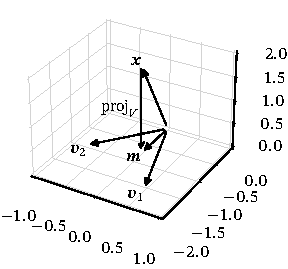
\includegraphics{figures/proj3d.pdf}
  \caption{\(\vect{x}\)の\(V=\spannedby\Set{\vect{v}_1,\vect{v}_2}\)への直交射影\(\vect{m}=\proj_V(\vect{x})\)の模式図.}
\end{figure}

\begin{example}[\(xy\)平面への直交射影]
  \(\vect{e}_x=\trps{\rowvect{1 & 0 & 0}}\),\(\vect{e}_y=\trps{\rowvect{0 & 1 & 0}}\)とし,
  \(\numset{R}^3\)の部分空間\(V\)を\(V=\spannedby\Set{\vect{e}_x,\vect{e}_y}\)で定義する.
  このとき,集合\(\Set{\vect{e}_x,\vect{e}_y}\)は\(V\)の正規直交基底なので\(\proj_V(\vect{r})=\innerp{\vect{r}}{\vect{e}_x}\vect{e}_x+\innerp{\vect{r}}{\vect{e}_y}\vect{e}_y=\trps{\rowvect{x & y & 0}}\)(\(\vect{r}=\trps{\rowvect{x & y & z}}\in\numset{R}^3\))である.
\end{example}

\begin{proposition}{}{}
  \(\numset{K}^n\)の任意の部分空間\(V\)について,写像\(\proj_V\colon\numset{K}^n\to V\)は線型写像である.
\end{proposition}

\begin{proof}
  \(s,t\in\numset{K}\),\(\vect{x},\vect{y}\in\numset{K}^n\)を任意にとり,\(\vect{z}=s\vect{x}+t\vect{y}\),\(\vect{m}=s\proj_V(\vect{x})+t\proj_V(\vect{y})\)とおく.
  このとき,任意の\(\vect{v}\in V\)に対して\(\innerp{\vect{z}-\vect{m}}{\vect{v}}=s\innerp{\vect{x}-\proj_V(\vect{x})}{\vect{v}}+t\innerp{\vect{y}-\proj_V(\vect{y})}{\vect{v}}=s0+t0=0\)なので,
  \(\proj_V(\vect{z})=\vect{m}\)である.よって,\(\proj_V\)は線型写像である.
\end{proof}

\subsection{直交補空間}

\begin{definition}{直交補空間}{numerical_perpendicular_complement}\index{ちょっこうほくうかん@直交補空間}\indexsymbol{\(\pcomp{V}\)}\indexsymbol{\(\pcomp[V]{W}\)}
  \(V\)を\(\numset{K}^n\)の部分空間とする.\(W\)が\(V\)の部分空間なら,集合
  \[
    \pcomp[V]{W} = \Set{\vect{v}\in V\given\text{任意の\(\vect{w}\in W\)に対して\(\innerp{\vect{v}}{\vect{w}}=0\)}}
  \]
  も\(V\)の部分空間になる.\(\pcomp[V]{W}\)を(\(V\)における)\(W\)の\termdef{直交補空間}(orthogonal complement)という.誤解のおそれがなければ,\(\pcomp[V]{W}\)を\(\pcomp{W}\)とも書く.
\end{definition}

\begin{example}
  \(W=\spannedby\Set{\vect{e}_1,\vect{e}_2}\)を\(\numset{R}^3\)の2次元部分空間とする.
  このとき,\(\numset{R}^3\)における\(W\)の直交補空間は,\(\vect{e}_1\)と\(\vect{e}_2\)に直交する\(\zvec\)でないベクトル\(\vect{e}_3\)で生成される直線\(\spannedby\Set{\vect{e}_3}\)である.
  特に\(\vect{e}_1\)と\(\vect{e}_2\)が直交するとき,集合\(\Set{\vect{e}_i/\vnorm{\vect{e}_i}\given i=1,2,3}\)は\(\numset{R}^3\)の正規直交基底である.
\end{example}

\begin{figure}[htbp]
  \centering
  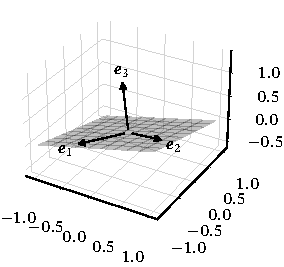
\includegraphics{figures/orthogonal_complement.pdf}
  \caption{\(W\)と\(\vect{e}_1\),\(\vect{e}_2\),\(\vect{e}_3\)の様子.}
\end{figure}

\begin{proposition}{}{}
  \(V\)は\(\numset{K}^n\)の部分空間で,\(W\)は\(V\)の部分空間とする.このとき\(V=W\oplus\pcomp[V]{W}\)である.
\end{proposition}

\begin{proof}
  \(\vect{x}\in W\cap\pcomp{W}\)なら\(\innerp{\vect{x}}{\vect{x}}=0\)なので\(\vect{x}=\zvec\),よって\(W\cap\pcomp{W}=\Set{\zvec}\)である.
  また\cref{proposition:finite_projection}より,任意の\(\vect{x}\in V\)に対して\(\vect{x}-\proj_W(\vect{x})\in\pcomp{W}\),\(\vect{x}=\proj_W(\vect{x})+(\vect{x}-\proj_W(\vect{x}))\in W+\pcomp{W}\)である.
  したがって\(V=W\oplus\pcomp{W}\)である.
\end{proof}

\subsection{分析と合成}

\cref{proposition:finite_convex_projection}の証明では,\(\proj_V(\vect{x})\)の存在を示すために\(V\)の正規直交基底\(\basis{B}=\Set{\vect{e}_1,\dots,\vect{e}_m}\)を1つ選び,\(\proj_V(\vect{x})\)を\(\sum_{i=1}^m\innerp{\vect{x}}{\vect{e}_i}\vect{e}_i\)と表した.
一方で(特に信号解析では),\(\vect{x}\)の性質を調べるのに利用したい\(\numset{C}^n\)の正規直交基底\(\basis{B}=\Set{\vect{e}_1,\dots,\vect{e}_n}\)があって,
そこから部分空間\(V_m=\spannedby\Set{\vect{e}_1,\dots,\vect{e}_m}\)(\(m=1,\dots,n\))への直交射影\(\proj_{V_m}(\vect{x})\)を作ることも多い.そのような場合,直交射影は3つの操作に分解できる.

\begin{definition}{エルミート転置}{hermitian_transpose}\index{えるみーとてんち@エルミート転置}\index{ずいはんぎょうれつ@随伴行列|see{エルミート転置}}\index{H@\(\htrps{\mat{A}}\)}
  \(\mat{A}\)を\(m\times n\)複素行列とする.\(n\times m\)行列\(\trps{\conj{\mat{A}}}\)を\(\mat{A}\)の\termdef{エルミート転置}(Hermitian transpose)といい,\(\htrps{\mat{A}}\)と表す\footnotemark .
\end{definition}

\footnotetext{エルミート転置は\termdef{随伴行列}(adjoint matrix)と呼ばれることも多いが,別の行列を随伴行列と呼ぶ流儀もあり,まぎらわしい.そのため,本書ではエルミート転置で統一する.}

\(\mat{U}=\htrps{\rowvect{\vect{e}_1 & \cdots & \vect{e}_n}}\),\(\mat{\Lambda}=\smallmatrice{\imat_m & \\ & \zmat_{n-m}}\)とおく(\(\imat_m\)は\(m\)次単位行列,\(\zmat_{n-m}\)は\(n-m\)次零行列).
このとき,任意の\(\vect{x}=\trps{\rowvect{x_1 & \cdots & x_n}}\in\numset{C}^n\)に対して
\[
  \mat{U}\vect{x} = \matrice*{\htrps{\vect{e}_1}\vect{x} \\ \vdots \\ \htrps{\vect{e}_n}\vect{x}}
  = \matrice*{\innerp{\vect{x}}{\vect{e}_1} \\ \vdots \\ \innerp{\vect{x}}{\vect{e}_n}},
  \quad\mat{\Lambda}\vect{x} = \matrice*{x_1 \\ \vdots \\ x_m \\ \zvec},
  \quad\htrps{\mat{U}}\vect{x} = \htrps{\mat{U}}\matrice*{x_1 \\ \vdots \\ x_n}
  = \sum_{i=1}^nx_i\vect{e}_i
\]
であるから
\[
  \htrps{\mat{U}}\mat{\Lambda}\mat{U}\vect{x} = \htrps{\mat{U}}\mat{\Lambda}\matrice*{\innerp{\vect{x}}{\vect{e}_1} \\ \vdots \\ \innerp{\vect{x}}{\vect{e}_n}}
  = \htrps{\mat{U}}\matrice*{\innerp{\vect{x}}{\vect{e}_1} \\ \vdots \\ \innerp{\vect{x}}{\vect{e}_m} \\ \zvec}
  = \sum_{i=1}^m\innerp{\vect{x}}{\vect{e}_i}\vect{e}_i
  = \proj_{V_m}(\vect{x})
\]
であり,\(\proj_{V_m}(\vect{x})=\htrps{\mat{U}}\mat{\Lambda}\mat{U}\vect{x}\)が成立する.言い換えれば,\(\proj_{V_m}\)は\(\numset{C}^n\)から\(\numset{C}^n\)への3つの線型写像
\(T(\vect{x})=\mat{U}\vect{x}\),\(L(\vect{x})=\mat{\Lambda}\vect{x}\),\(\synth{T}(\vect{x})=\htrps{\mat{U}}\vect{x}\)を用いて,\(\proj_{V_m}=\synth{T}LT\)と表せる.

\(T(\vect{x})\)の第\(i\)成分\(\innerp{\vect{x}}{\vect{e}_i}\)は,\(\vect{x}\)に含まれる\(\vect{e}_i\)の「成分」を表すと考えられる.その理由は2つある.
1つめの理由は,\(\vnorm{\proj_{\spannedby\Set{\vect{e}_i}}(\vect{x})}=\vnorm{\innerp{\vect{x}}{\vect{e}_i}\vect{e}_i}=\abs{\innerp{\vect{x}}{\vect{e}_i}}\)なので,
\(\abs{\innerp{\vect{x}}{\vect{e}_i}}\)が\(\vect{e}_i\)のスカラー倍で\(\vect{x}\)を最もよく近似するベクトルの長さを表すことである.
もう1つの理由は,\(\basis{B}\)は\(\numset{K}^n\)の正規直交基底であるから
\begin{equation}
  \label{equation:analysis_and_synthesis}
  \vect{x} = \proj_{V_n}(\vect{x})
  = \sum_{i=1}^n\innerp{\vect{x}}{\vect{e}_i}\vect{e}_i
\end{equation}
が成立し,\(\innerp{\vect{x}}{\vect{e}_i}\vect{e}_i\)の和で\(\vect{x}\)が表されることである.

以上の理由から,本書では線型写像\(T(\vect{x})=\trps{\rowvect{\innerp{\vect{x}}{\vect{e}_1} & \cdots & \innerp{\vect{x}}{\vect{e}_n}}}\)を分析作用素,\(\synth{T}(\vect{x})=\sum_{i=1}^nx_i\vect{e}_i\)を合成作用素と呼ぶ.

\begin{definition}{分析作用素,合成作用素}{analysis_and_synthesis}\index{ぶんせきさようそ@分析作用素}\index{ごうせいさようそ@合成作用素}
  \(\basis{B}=\Set{\vect{e}_1,\dots,\vect{e}_n}\)を\(\numset{K}^n\)の正規直交基底とする.
  \begin{enumerate}
    \item 線型写像\(T\colon\numset{K}^n\to\numset{K}^n\),\(T(\vect{x})=\trps{\rowvect{\innerp{\vect{x}}{\vect{e}_1} & \cdots & \innerp{\vect{x}}{\vect{e}_n}}}\)を\(\basis{B}\)に関する\termdef{分析作用素}(analysis operator)という.
    \item 線型写像\(\synth{T}\colon\numset{K}^n\to\numset{K}^n\),\(\synth{T}(\trps{\rowvect{x_1 & \cdots & x_n}})=\sum_{i=1}^nx_i\vect{e}_i\)を\(\basis{B}\)に関する\termdef{合成作用素}(synthesis operator)という.
  \end{enumerate}
\end{definition}

\cref{equation:analysis_and_synthesis}より,合成作用素は分析作用素の逆写像である.
また,分析作用素と合成作用素が持つ性質は,表現行列に関する条件へと言い換えられる.

\begin{definition}{正規行列,ユニタリ行列}{regular_and_unitary_matrix}\index{せいきぎょうれつ@正規行列}\index{ゆにたりぎょうれつ@ユニタリ行列}
  \(\mat{A}\)を\(n\)次複素正方行列とする.
  \begin{enumerate}
    \item \(\htrps{\mat{A}}\mat{A}=\mat{A}\htrps{\mat{A}}\)であるとき,\(\mat{A}\)を\termdef{正規行列}(normal matrix)という.
    \item \(\htrps{\mat{A}}\mat{A}=\mat{A}\htrps{\mat{A}}=\imat\)であるとき(つまり\(\htrps{\mat{A}}=\mat{A}^{-1}\)であるとき),\(\mat{A}\)を\termdef{ユニタリ行列}(unitary matrix)という.
  \end{enumerate}
\end{definition}

正規行列とユニタリ行列の関係については\cref{section:least_square}で詳述することにして,ここでは次の命題を示す.

\begin{proposition}{ユニタリ行列の性質}{}
  \(\mat{U}=\rowvect{\vect{u}_1 & \cdots & \vect{u}_n}\)を\(n\)次複素正方行列とする.このとき,\(\mat{U}\)に関する以下の条件は同値である.
  \begin{enumerate}
    \item \(\mat{U}\)はユニタリ行列である.
    \item 集合\(\Set{\vect{u}_1,\dots,\vect{u}_n}\)は\(\numset{C}^n\)の正規直交基底である.
  \end{enumerate}
\end{proposition}

\begin{proof}
\[
  \htrps{\mat{U}}\mat{U} = \matrice*{\htrps{\vect{u}_1} \\ \vdots \\ \htrps{\vect{u}_n}}\matrice{\vect{u}_1 & \cdots & \vect{u}_n}
   = \matrice*{\htrps{\vect{u}_1}\vect{u}_1 & \cdots & \htrps{\vect{u}_1}\vect{u}_n \\ \vdots & \ddots & \vdots \\ \htrps{\vect{u}_n}\vect{u}_1 & \cdots & \htrps{\vect{u}_n}\vect{u}_n}
 \]
  なので,\(\htrps{\vect{u}_i}{\vect{u}_j}=\conj*{\innerp{\vect{u}_i}{\vect{u}_j}}=\kdelta{i}{j}\)がすべての\(i,j\in\Set{1,\dots,n}\)に対して成り立つことは,\(\htrps{\mat{U}}\mat{U}=\imat\)と同値である.
\end{proof}

\begin{corollary}{}{}
  \(T\colon\numset{C}^n\to\numset{C}^n\)を線型写像とする.このとき,\(T\)に関する以下の条件は同値である.
  \begin{enumerate}
    \item \(T\)はある正規直交基底に関する分析作用素(合成作用素)である.
    \item 標準基底に関する\(T\)の表現行列はユニタリ行列である.
  \end{enumerate}
\end{corollary}

\section{離散フーリエ変換}

この節から,本書の主題である信号解析に入っていく.

\subsection{離散フーリエ変換}

\begin{definition}{離散フーリエ変換}{discrete_fourier_transform}\index{りさんふーりえへんかん@離散フーリエ変換!かずべくとる@数ベクトル}\index{DFT|see{離散フーリエ変換}}\index{FZN@\(\dft{N}\)}
  各\(\vect{x}=\trps{\rowvect{x_0 & \cdots & x_{N-1}}}\in\numset{C}^N\)に対して,\(\numset{C}^N\)の元
  \[
    \vect{\hat{x}} = \trps{\matrice{\hat{x}_0 & \cdots & \hat{x}_{N-1}}},
    \quad\hat{x}_k = \frac{1}{\sqrt{N}}\sum_{n=0}^{N-1}x_n\napr^{-2\krez\iuni kn/N}
  \]
  を対応づける線型写像\(\dft{N}\colon\numset{C}^N\to\numset{C}^N\)を\termdef{離散フーリエ変換}(Discrete Fourier transform; DFT)という.
\end{definition}

以下では\(\napr^{2\krez\iuni/N}=\cos(2\krez/N)+\iuni\sin(2\krez/N)\)を単に\(\zeta\)と書く.

\begin{proposition}{}{dft_onb}
  \(\vect{w}_k=N^{-1/2}\trps{\rowvect{\zeta^{k\cdot 0} & \cdots & \zeta^{k(N-1)}}}\)とする.
  このとき,集合\(\Set{\vect{w}_0,\dots,\vect{w}_{N-1}}\)は\(\numset{C}^N\)の正規直交基底である.
\end{proposition}

\begin{proof}
  \(\conj{\zeta}=\zeta^{-1}\)だから,\(\innerp{\vect{w}_i}{\vect{w}_j}=\trps{\vect{w}_i}\conj{\vect{w}}_j\)は
  \[
    \sum_{n=0}^{N-1}\frac{\zeta^{in}}{\sqrt{N}}\frac{\conj{\zeta}^{jn}}{\sqrt{N}} = \frac{1}{N}\sum_{n=0}^{N-1}\zeta^{(i-j)n}
    = \begin{cases}(\zeta^{(i-j)N}-1)/(N(\zeta^{i-j}-1)) & (i\neq j), \\ 1 & (i=j)\end{cases}
  \]
  と変形できる.\(\zeta^N=1\)なので\(\innerp{\vect{w}_i}{\vect{w}_j}=\kdelta{i}{j}\)である.
\end{proof}

\cref{proposition:dft_onb}から,\(\dft{N}\)は正規直交基底\(\basis{W}=\Set{\vect{w}_0,\dots,\vect{w}_{N-1}}\)に関する分析作用素である.
分析作用素の逆写像は合成作用素なので,\(\dft{N}\)の逆変換は
\begin{equation}
  \label{equation:idft}
  \vect{x} = \sum_{k=0}^{N-1}\hat{x}_k\vect{w}_k,
  \quad x_n = \frac{1}{\sqrt{N}}\sum_{k=0}^{N-1}\hat{x}_k\napr^{2\krez\iuni kn/N}
\end{equation}
と書ける.

\begin{proposition}{}{dft_plancherel}
  \(\vect{\hat{x}}=\dft{N}\vect{x}\),\(\vect{\hat{y}}=\dft{N}\vect{y}\)とすると,\(\innerp{\vect{\hat{x}}}{\vect{\hat{y}}}=\innerp{\vect{x}}{\vect{y}}\)が成立する.
\end{proposition}

\begin{proof}
  標準基底に関する\(\dft{N}\)の表現行列を\(\mat{W}\)とおく.このとき
  \(\innerp{\vect{\hat{x}}}{\vect{\hat{y}}}=\innerp{\mat{W}\vect{x}}{\vect{\hat{y}}}=\trps{\vect{x}}\trps{\mat{W}}\conj{\vect{\hat{y}}}=\trps{\vect{x}}\conj*{\htrps{\mat{W}}\vect{\hat{y}}}=\innerp{\vect{x}}{\htrps{\mat{W}}\vect{\hat{y}}}\)
  であり,\(\mat{W}\)はユニタリ行列なので\(\htrps{\mat{W}}\vect{\hat{y}}=\htrps{\mat{W}}\mat{W}\vect{y}=\vect{y}\),\(\innerp{\vect{x}}{\htrps{\mat{W}}\vect{\hat{y}}}=\innerp{\vect{x}}{\vect{y}}\)となる.
\end{proof}

\cref{proposition:dft_plancherel}に関して,特に\(\vect{x}=\vect{y}\)のとき
\begin{equation}
  \label{equation:dft_parseval}
  \vnorm{\dft{N}\vect{x}}^2 = \vnorm{\vect{x}}^2,
  \quad\sum_{k=0}^{N-1}\abs{\hat{x}_k}^2 = \sum_{n=0}^{N-1}\abs{x_n}^2
\end{equation}
である.信号処理ではしばしば\cref{equation:dft_parseval}を\termdef{パーセヴァルの定理}\index{ぱーせばるのていり@パーセヴァルの定理}(Parseval's theorem),あるいは\termdef{プランシュレルの定理}\index{ぷらんしゅれるのていり@プランシュレルの定理}(Plancherel's theorem)と呼ぶ.

他の諸性質を導く前に,離散フーリエ変換の工学的重要性を見ておこう.

\begin{figure}[htbp]
  \centering
  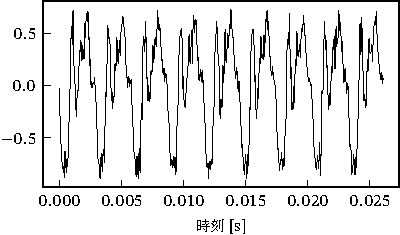
\includegraphics{figures/time_domain.pdf}
  \caption{「あ」の波形.}
  \label{figure:time_domain}
\end{figure}

\begin{wrapfigure}[10]{o}{0pt}
  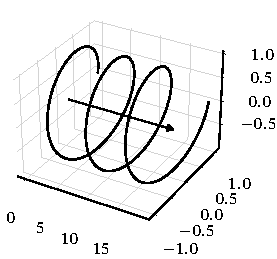
\includegraphics{figures/helix.pdf}
\end{wrapfigure}

\cref{figure:time_domain}は「あ」という音声の波形である\footnote{出典は波音リツ単独音 Ver1.5.1 \cite{canon}.}.
\cref{section:numerical_vector_space_introduction}で述べたように,\cref{figure:time_domain}のデータは数ベクトル\(\vect{x}\in\numset{R}^N\)と見なせる.
そして,分析作用素に関する考察によれば,\(\hat{x}_k=\innerp{\vect{x}}{\vect{w}_k}\)は\(\vect{x}\)に含まれる\(\vect{w}_k\)の成分に相当する.
つまり,\(\hat{x}_k\)の絶対値\(\abs{\hat{x}_k}\)は音声\(\vect{x}\)に含まれる\(\vect{w}_k\)の量を表すと考えられる.では,偏角\(\arg\hat{x}_k\)はどういう意味を持つのだろう\?極形式\(\hat{x}_k=\abs{\hat{x}_k}\napr^{\iuni\arg\hat{x}_k}\)を\cref{equation:idft}に代入すると
\[
  x_n = \frac{1}{\sqrt{N}}\sum_{k=0}^{N-1}\hat{x}_k\napr^{2\krez\iuni kn/N}
  = \frac{1}{\sqrt{N}}\sum_{k=0}^{N-1}\abs{\hat{x}_k}\napr^{\iuni(2\krez kn/N+\arg\hat{x}_k)}
\]
となるから,\(\arg\hat{x}_k\)は音声\(\vect{x}\)に含まれる周波数\(k/N\)の波\(\sqrt{N}\midx{w}{k}{n}=\napr^{2\krez\iuni kn/N}\)の初期位相を表している.この波は図のような螺旋形を描く(矢印は時間軸).

実際に\(\abs{\hat{x}_k}\)を計算すると,\cref{figure:frequency_domain}実線部のようになる.

\begin{figure}[htbp]
  \centering
  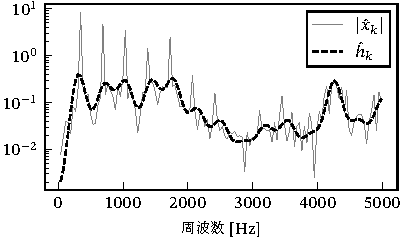
\includegraphics{figures/frequency_domain.pdf}
  \caption{「あ」の離散フーリエ変換.}
  \label{figure:frequency_domain}
\end{figure}

\cref{figure:frequency_domain}を見ると,\SI{350}{Hz}周辺に1つめのピークが現れている.これは\termdef{基本周波数}\index{きほんしゅうはすう@基本周波数}(fundamental frequency)と呼ばれる量で,
人間が知覚する声の高さとかなりよく対応する\index{ピッチ}\footnote{人間が知覚する声の高さを\termdef{ピッチ}(pitch)という.ピッチと基本周波数は多くの場合対応するが,同一視できないケースも存在する\cite{kashino}.}.

また,\cref{figure:frequency_domain}の破線部\(\hat{h}_k\)は,基本周波数に起因する細かな変動を\(\abs{\hat{x}_k}\)から除いた曲線である.
この曲線は\termdef{スペクトル包絡}\index{すぺくとるほうらく@スペクトル包絡}(spectral envelope)といい,音声の音色とよく対応する.
つまり,離散フーリエ変換を使うことで,音声が持つ基本周波数(\(\mathord{\fallingdotseq}\text{声の高さ}\))由来の性質と,スペクトル包絡(\(\mathord{\fallingdotseq}\text{音色}\))由来の性質を分離して解析できる.

\subsection{エイリアシング}

さきほど「\(\sqrt{N}\midx{w}{k}{n}=\napr^{2\krez\iuni kn/N}\)は周波数\(k/N\)の波である」と述べたが,この表現には少し語弊がある.

周波数\(f\,\si{Hz}\)の波\(\napr^{2\krez\iuni ft}\)について,瞬時値を1秒あたり\(f_{\symrm{s}}\)回記録すると数列\(\seq{\napr^{2\krez\iuni fn/f_{\symrm{s}}}}_{n\in\numset{Z}}\)ができる.
一方,周波数\(f-f_{\symrm{s}}\,\si{Hz}\)の波\(\napr^{2\krez\iuni(f-f_{\symrm{s}})t}\)について,同じ方法で数列を作ると,その一般項は
\[
  \napr^{2\krez\iuni(f-f_{\symrm{s}})n/f_{\symrm{s}}} = \napr^{2\krez\iuni fn/f_{\symrm{s}}-2\krez\iuni n}
  = \napr^{2\krez\iuni fn/f_{\symrm{s}}}(\napr^{-2\krez\iuni})^n
  = \napr^{2\krez\iuni fn/f_{\symrm{s}}}
\]
となる.つまり,周波数が\(f\,\si{Hz}\)でも\(f-f_{\symrm{s}}\,\si{Hz}\)でも,できる数列は変わらない.

言い換えると,周波数が\(f_{\symrm{s}}\)だけ異なる波は数列から区別できない.\cref{figure:aliasing}は\(f_{\symrm{s}}=\SI{2.5}{Hz}\)のとき,
周波数\SI{2}{Hz}の波\(\sin(4\krez t)\)と\SI{-0.5}{Hz}の波\(\sin(-\krez t)\)が,時刻\(n/f_{\symrm{s}}\)秒(\(n\in\numset{Z}\))では同じ瞬時値を持つことを示している.

\begin{figure}[htbp]
  \centering
  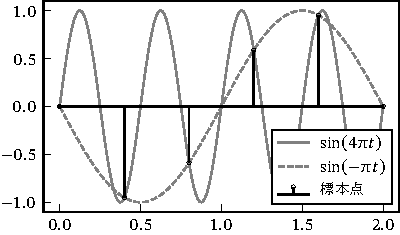
\includegraphics{figures/aliasing.pdf}
  \caption{エイリアシングの様子.}
  \label{figure:aliasing}
\end{figure}

一般に,連続時間の信号から離散時間の信号を得る操作を\termdef{標本化}\index{ひょうほんか@標本化}\index{サンプリング|see{標本化}}(sampling)といい,標本化によって信号が区別できなくなる現象を\termdef{エイリアシング}\index{エイリアシング}(aliasing)という.
また,\(f_{\symrm{s}}\)を\termdef{標本化周波数}\index{ひょうほんかしゅうはすう@標本化周波数}(sampling frequency)という.

\cref{figure:aliasing}の場合,標本化後の信号は周波数の絶対値が小さい(つまり低周波である)\SI{-0.5}{Hz}の波を表すと考えるほうが自然だろう.
周波数\(f\)の波を標本化すると,\(f\)より低周波の波と区別できなくなるのは\(\abs{f}\geq f_{\symrm{s}}/2\)のときである.\(f_{\symrm{s}}/2\)のことを\termdef{ナイキスト周波数}\index{ないきすとしゅうはすう@ナイキスト周波数}(Nyquist frequency)という.

話を離散フーリエ変換に戻すと,\(\sqrt{N}\midx{w}{k}{n}=\napr^{2\krez\iuni kn/N}\)は\(f=k\)の波が\(f_{\symrm{s}}=N\)で標本化されたものとみなせる.
そのため,\(k\geq N/2\)のとき\(\sqrt{N}\midx{w}{k}{n}\)は周波数\(k/N\)の波ではなく,周波数\((k-N)/N\)の波を表すとみなすのが普通である.

\subsection{巡回畳み込み}

以下に\cref{equation:idft}を再掲する.
\[
  x_n = \frac{1}{\sqrt{N}}\sum_{k=0}^{N-1}\hat{x}_k\napr^{2\krez\iuni kn/N}
\]

\cref{equation:idft}は本来,\(\vect{x}=\trps{\rowvect{x_0 & \cdots & x_{N-1}}}\)を\(\vect{\hat{x}}=\dft{N}\vect{x}\)によって表す式である.
しかし,それをひとまず忘れて\(n\)に任意の整数を代入すれば,\(\vect{x}\)を周期\(N\)の数列\(\seq{x[n]}_{n\in\numset{Z}}\)へと拡張できる.
そこで,周期\(N\)の複素数列\(x=\seq{x[n]}_{n\in\numset{Z}}\)に対して\(\hat{x}=\dft{N}x\)を次のように定義する.

\begin{definition}{}{cycle_dft}\index{りさんふーりえへんかん@離散フーリエ変換!しゅうきすうれつ@周期数列}\indexsymbol{\(\cycles{\numset{C}}{N}\)}\index{FZN@\(\dft{N}\)}
  周期\(N\)の複素数列全体\(\Set{\seq{u[i]}_{i\in\numset{Z}}\given u[i]=u[i+N]\in\numset{C}}\)を\(\cycles{\numset{C}}{N}\)と表記する\footnotemark .
  線型写像\(\dft{N}\colon\cycles{\numset{C}}{N}\to\cycles{\numset{C}}{N}\)を次式で定義する.
  \[
    (\dft{N}x)[k] =  \frac{1}{\sqrt{N}}\sum_{n=0}^{N-1}x[n]\napr^{-2\krez\iuni kn/N}\quad(x\in\cycles{\numset{C}}{N})
  \]
\end{definition}

\footnotetext{信号処理では,数列の添字\texttwoemdash すなわち,離散的な集合で定義された関数の引数\texttwoemdash を大かっこで表す慣例がある.}
\(\cycles{\numset{C}}{N}\)は加法\(x+y=\seq{x[n]+y[n]}\),スカラー乗法\(\lambda x=\seq{\lambda x[n]}\)に関する\(N\)次元ベクトル空間である.

はじめに定義した離散フーリエ変換と\cref{definition:cycle_dft}の\(\dft{N}\)は,ある意味「同じもの」と見なせる.実際,数列
\[
  \delta_i[n] = \sum_{m\in\numset{Z}}\kdelta{n}{(mN+i)}
  = \begin{cases}1 & (n\equiv i\pmod{N}),\\ 0 & \text{(otherwise)}\end{cases}\quad(0\leq i<N)
\]
からなる集合\(\basis{D}=\Set{\delta_0,\dots,\delta_{N-1}}\)は\(\cycles{\numset{C}}{N}\)の基底であり,\(\numset{C}^N\)の標準基底と\(\basis{D}\)を対応づければ,2つの\(\dft{N}\)を同一視できる.

\begin{note}
形式ばらずにいえば,数列\(x\)の周期が\(N\)なら,\(x\)の様子は時刻\(N-1\)までのデータ\(\phi(x)=\trps{\rowvect{x[0] & \cdots & x[N-1]}}=\sum_{i=0}^{N-1}x[i]\vect{e}_i\)から解析できるし,\(\phi(x)\)から\(x\)を復元するのも容易である.この対応を
\[
  \sum_{i=0}^{N-1}x_i\delta_i \stackrel{\phi}{\longleftrightarrow} \sum_{i=0}^{N-1}x_i\vect{e}_i
\]
と表すと,\(\dft{N}\)は\(\stackrel{\phi}{\longleftrightarrow}\)を保ち,次式が成立する(\cref{subsection:representation_matrix}を見よ).
\[
  \dft{N}\pqty*{\sum_{i=0}^{N-1}x_i\delta_i} = \sum_{i=0}^{N-1}x_i\hat{\delta}_i
  \stackrel{\phi}{\longleftrightarrow} \sum_{i=0}^{N-1}x_i\vect{\hat{e}}_i
  = \dft{N}\pqty*{\sum_{i=0}^{N-1}x_i\vect{e}_i}
\]
\end{note}

ベクトル空間\(\cycles{\numset{C}}{N}\)において,\termdef{ラグ作用素}\index{らぐさようそ@ラグ作用素}(lag operator)\(\lagop\)を\(\lagop x=\seq{x[n-1]}\)で定義する.
このとき,\cref{proposition:dft_shift_theorem}が成立する.

\begin{proposition}{}{dft_shift_theorem}
  任意の\(x\in\cycles{\numset{C}}{N}\)に対して\((\dft{N}\lagop x)[k]=\zeta^{-k}\hat{x}[k]\)である.
\end{proposition}

\begin{proof}
  \(\sum\)の添字\(n\)を\(m=n+1\)に置き換えると
  \[
    \zeta^{-k}\hat{x}[k] = \frac{1}{\sqrt{N}}\sum_{n=0}^{N-1}x[n]\napr^{-2\krez\iuni k(n+1)/N}
    = \frac{1}{\sqrt{N}}\sum_{m=1}^Nx[m-1]\napr^{-2\krez\iuni km/N}
  \]
  となる.右辺は周期数列の1周期に渡る和だから,\(\sum_{m=1}^N\)を\(\sum_{m=0}^{N-1}\)に変えても値は変わらない.よって\(\zeta^{-k}\hat{x}[k]=(\dft{N}\lagop x)[k]\)である.
\end{proof}

\cref{proposition:dft_shift_theorem}を使うと,数列の積\(x\cdot y=\seq{x[n]y[n]}\)と離散フーリエ変換の間にある関係を示せる.積は\(\dft{N}\)で,次の2項演算へと写される.

\begin{definition}{巡回畳み込み}{}\index{じゅんかいたたみこみ@巡回畳み込み}\index{たたみこみ@畳み込み!じゅんかい@巡回}\indexsymbol{\(x\circconv y\)}
  \(x,y\in\cycles{\numset{C}}{N}\)とする.次式で定義される\(z\in\cycles{\numset{C}}{N}\)を\(x\)と\(y\)の\termdef{巡回畳み込み}(circular convolution)といい,\(x\circconv y\)と表記する.
  \[
    z[n] = \sum_{m=0}^{N-1}x[m]y[n-m]\quad(n\in\numset{Z})
  \]
\end{definition}

\begin{proposition}{}{dft_convolution_theorem}
  任意の\(x,y\in\cycles{\numset{C}}{N}\)に対して次式が成立する.
  \[
    \dft{N}(x\circconv y) = \sqrt{N}\hat{x}\cdot\hat{y},
    \quad\dft{N}(x\cdot y) = \frac{1}{\sqrt{N}}\hat{x}\circconv\hat{y}
  \]
\end{proposition}

\begin{proof}
  1つめのみ示す.\(z=x\circconv y\)とし,\(\sum_n\)と\(\sum_m\)を交換すると
  \begin{align*}
    (\dft{N}z)[k] &= \frac{1}{\sqrt{N}}\sum_{n=0}^{N-1}\pqty*{\sum_{m=0}^{N-1}x[m]y[n-m]}\zeta^{-kn} \\
    &= \sum_{m=0}^{N-1}x[m]\pqty*{\frac{1}{\sqrt{N}}\sum_{n=0}^{N-1}y[n-m]\zeta^{-kn}}
  \end{align*}
  となる.\cref{proposition:dft_shift_theorem}より\((\dft{N}\lagop^my)[k]=\zeta^{-mk}\hat{y}[k]\)なので
  \[
    (\dft{N}z)[k] = \sum_{m=0}^{N-1}x[m](\zeta^{-mk}\hat{y}[k])
    = \sqrt{N}\pqty*{\frac{1}{\sqrt{N}}\sum_{m=0}^{N-1}x[m]\zeta^{-km}}\hat{y}[k]
  \]
  である.よって\((\dft{N}z)[k]=\sqrt{N}\hat{x}[k]\hat{y}[k]\)である.
\end{proof}

\begin{corollary}{}{circular_convolution_properties}
  任意の\(x,y,z\in\cycles{\numset{C}}{N}\)に対して,以下の式が成立する.
  \begin{enumerate}
    \item \(x\circconv y=y\circconv x\)
    \item \((x\circconv y)\circconv z=x\circconv (y\circconv z)\)
    \item \(x\circconv(y+z)=(x\circconv y)+(x\circconv z)\)
  \end{enumerate}
\end{corollary}

\begin{proof}
  2つめのみ示す.\(\dft{N}(x\circconv (y\circconv z))=\sqrt{N}\hat{x}\cdot\dft{N}(y\circconv z)=N\hat{x}\cdot(\hat{y}\cdot\hat{z})\)より
  \(x\circconv(y\circconv z)=N\dft{N}^{-1}(\hat{x}\cdot\hat{y}\cdot\hat{z})\)であり,同じ計算によって\((x\circconv y)\circconv z=N\dft{N}^{-1}(\hat{x}\cdot\hat{y}\cdot\hat{z})\)も確かめられる.
\end{proof}

最後に,\(\cycles{\numset{C}}{N}\)上で得られた結果を\(\numset{C}^N\)上のものに変換しよう.
\(h\in\cycles{\numset{C}}{N}\)を任意にとり,線型写像\(H\colon\cycles{\numset{C}}{N}\to\cycles{\numset{C}}{N}\)を\(H(x)=h\circconv x\)で定義する.
基底\(\basis{D}\)に関する\(H\)の表現行列\(\mat{H}\)は
\[
  \mat{H} = \matrice*{h[0] & h[N-1] & h[N-2] & \cdots & h[2] & h[1] \\ h[1] & h[0] & h[N-1] & \cdots & h[3] & h[2] \\ h[2] & h[1] & h[0] & \cdots & h[4] & h[3] \\ \vdots & \vdots & \vdots & \ddots & \vdots & \vdots \\ h[N-2] & h[N-3] & h[N-4] & \cdots & h[0] & h[N-1] \\  h[N-1] & h[N-2] & h[N-3] & \cdots & h[1] & h[0]}
\]
という形をしている.この形の行列を\termdef{巡回行列}\index{じゅんかいぎょうれつ@巡回行列}(circulant matrix)という.

同様に,基底\(\basis{D}\)に関する\(\dft{N}\)の表現行列を\(\mat{W}\)とおく.\(\mat{W}\)は\(\numset{C}^N\)上で定義した\(\dft{N}\)の,標準基底に関する表現行列でもある.

\begin{proposition}{}{}
  巡回行列は離散フーリエ変換で対角化される.すなわち,任意の\(N\)次巡回行列\(\mat{H}\)について\(\mat{W}\mat{H}\mat{W}^{-1}\)は対角行列である.
\end{proposition}

\begin{proof}
  \(\mat{H}\)の第1列を\(\trps{\rowvect{h_0 & \cdots & h_{N-1}}}\)とおき,\(\cycles{\numset{C}}{N}\)上の線型写像\(H\),\(\hat{H}\)をそれぞれ
  \(H(x)=h\circconv x\),\(\hat{H}(x)=\hat{h}\cdot x\)(\(h=\sum_{i=0}^{N-1}h_i\delta_i\))で定義する.\cref{proposition:dft_convolution_theorem}より
  \[
    (\dft{N}H\dft{N}^{-1})x = \dft{N}(h\circconv\dft{N}^{-1}x)
    = \hat{h}\cdot x
    = \hat{H}(x)\quad(x\in\cycles{\numset{C}}{N})
  \]
  だから,基底\(\basis{D}\)に関する\(\hat{H}\)の表現行列\(\mat{\hat{H}}=\diag(\hat{h}[0],\dots,\hat{h}[N-1])\)は,\(\dft{N}H\dft{N}^{-1}\)の表現行列\(\mat{W}\mat{H}\mat{W}^{-1}\)に一致する.
\end{proof}

\subsection{多次元離散フーリエ変換}

\begin{definition}{多次元離散フーリエ変換}{multidimensional_discrete_fourier_transform}\index{りさんふーりえへんかん@離散フーリエ変換!たじげん@多次元}\index{FZdn@\(\dft[d]{\vect{n}}\)}
  \(\vect{n}=\trps{\rowvect{N_1 & \cdots & N_d}}\)を自然数の組とし,\(\Omega=\Set{\trps{\rowvect{u_1 & \cdots & u_d}}\given\text{\(u_i\in\numset{Z}\),\(0\leq u_i<N_i\)(\(1\leq i\leq d\))}}\),\(\mat{N}=\diag(N_1,\dots,N_d)\)とおく.
  関数\(x\colon\Omega\to\numset{C}\)に対して,関数
  \[
    \hat{x}[\vect{k}] = \frac{1}{\sqrt{\det\mat{N}}}\sum_{\vect{r}\in\Omega}x[\vect{r}]\napr^{-2\krez\iuni\trps{\vect{k}}\mat{N}^{-1}\vect{r}}\quad(\vect{k}\in\Omega)
  \]
  を対応づける線型写像\(\dft[d]{\vect{n}}\colon\numset{C}^\Omega\to\numset{C}^\Omega\)を\termdef{\(d\)次元離散フーリエ変換}という.
\end{definition}

特に\(d=2\)のとき
\begin{align*}
  \hat{x}[k_1,k_2] &= \frac{1}{\sqrt{N_1N_2}}\sum_{r_2=0}^{N_2-1}\sum_{r_1=0}^{N_1-1}x[r_1,r_2]\napr^{-2\krez\iuni(k_1r_1/N_1+k_2r_2/N_2)} \\
  &= \frac{1}{\sqrt{N_2}}\sum_{r_2=0}^{N_2-1}\pqty*{\frac{1}{\sqrt{N_1}}\sum_{r_1=0}^{N_1-1}x[r_1,r_2]\napr^{-2\krez\iuni k_1r_1/N_1}}\napr^{-2\krez\iuni k_2r_2/N_2}
\end{align*}
であり,右辺は\(x[r_1,r_2]\)を各変数に関して離散フーリエ変換した形になっている.
より一般に,\(x[r_1,\dots,r_d]\)の\(d\)次元離散フーリエ変換は,\(x[r_1,\dots,r_d]\)を各変数に関して離散フーリエ変換したものと一致する.

次の命題は,一般の次元で離散フーリエ変換が分析作用素であることを示している.
ただし,\(\numset{C}^\Omega\)の内積は1変数のときと同様\(\innerp{x}{y}=\sum_{\vect{r}\in\Omega}x[\vect{r}]\conj*{y[\vect{r}]}\)で定義する.

\begin{proposition}{}{}
  \(w_{\vect{k}}[\vect{r}]=(\det\mat{N})^{-1/2}\exp(2\krez\iuni\trps{\vect{k}}\mat{N}^{-1}\vect{r})\)とする.このとき,集合\(\Set{w_{\vect{k}}\given\vect{k}\in\Omega}\)は\(\numset{C}^\Omega\)の正規直交基底である.
\end{proposition}

\begin{figure}[htbp]
  \begin{minipage}{\linewidth/2}
    \centering
    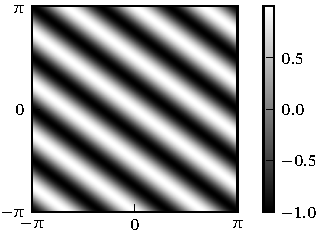
\includegraphics{figures/2dcos.pdf}
    \end{minipage}%
  \begin{minipage}{\linewidth/2}
    \centering
    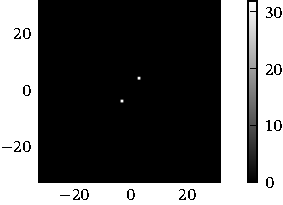
\includegraphics{figures/2dcos_dft.pdf}
  \end{minipage}
  \caption{\(\cos(3x+4y)\)のグラフと2次元離散フーリエ変換.}
\end{figure}

\begin{figure}[htbp]
  \begin{minipage}{\linewidth/2}
    \centering
    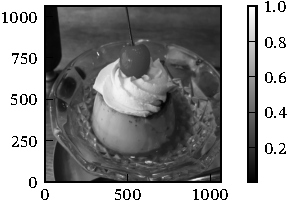
\includegraphics{figures/pudding.pdf}
  \end{minipage}%
  \begin{minipage}{\linewidth/2}
    \centering
    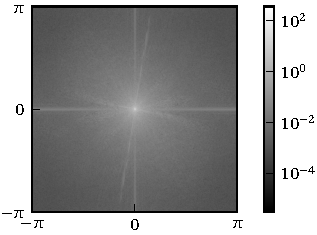
\includegraphics{figures/pudding_dft.pdf}
  \end{minipage}
  \caption{画像の2次元離散フーリエ変換.}
\end{figure}

\section{最小2乗問題}
\label{section:least_square}

本節では,直交射影の理論を近似へと応用する.

\subsection{最小2乗問題}

\subsection{スペクトル定理}

\subsection{特異値分解}

\subsection{擬似逆行列}

\section{多重解像度解析}

\section{主成分分析}

\begin{figure}[htbp]
  \begin{minipage}{\linewidth/2}
    \centering
    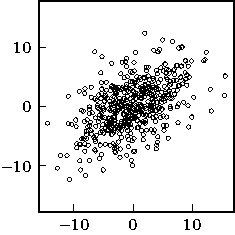
\includegraphics{figures/scatter.pdf}
  \end{minipage}%
  \begin{minipage}{\linewidth/2}
    \centering
    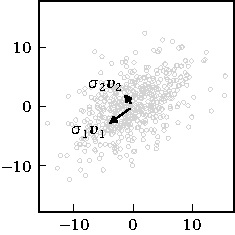
\includegraphics{figures/pca.pdf}
  \end{minipage}
\end{figure}

\begin{subappendices}
\section{窓関数}

\section{低ランク近似}

\end{subappendices}

\section*{演習問題}
\addcontentsline{toc}{section}{演習問題}

\begin{enumerate}
  \item 環\((\cycles{\numset{C}}{N},+,\circconv)\)は\(\numset{C}[x]/\langle x^N-1\rangle\)と同型であることを示せ.
\end{enumerate}

\end{document}
